% Standard Article Definition
\documentclass[]{article}

% Page Formatting
\usepackage[margin=1in]{geometry}
\setlength\parindent{0pt}

% Graphics
\usepackage{graphicx}

% Math Packages
\usepackage{physics}
\usepackage{amsmath, amsfonts, amssymb, amsthm}
\usepackage{mathtools}

% Extra Packages
\usepackage{pdfpages}
\usepackage{hyperref}
% \usepackage{listings}

% Section Heading Settings
\usepackage{enumitem}
% \renewcommand{\theenumi}{\alph{enumi}}
\renewcommand*{\thesection}{Problem \arabic{section}}
\renewcommand*{\thesubsection}{\alph{subsection})}
\renewcommand*{\thesubsubsection}{}%\quad \quad \roman{subsubsection})}

\newcommand{\Problem}{\subsubsection*{\textbf{PROBLEM:}}}
\newcommand{\Solution}{\subsubsection*{\textbf{SOLUTION:}}}
\newcommand{\Preliminaries}{\subsubsection*{\textbf{PRELIMINARIES:}}}

%Custom Commands
\newcommand{\N}{\mathbb{N}}
\newcommand{\Z}{\mathbb{Z}}
\newcommand{\Q}{\mathbb{Q}}
\newcommand{\R}{\mathbb{R}}
\newcommand{\C}{\mathbb{C}}

\newcommand{\SigAlg}{\mathcal{S}}

\newcommand{\Rel}{\mathcal{R}}

% \newcommand{\toI}{\xrightarrow{\textsf{\tiny I}}}
% \newcommand{\toS}{\xrightarrow{\textsf{\tiny S}}}
% \newcommand{\toB}{\xrightarrow{\textsf{\tiny B}}}

\newcommand{\divisible}{ \ \vdots \ }
\newcommand{\st}{\ : \ }

% Theorem Definition
\newtheorem{definition}{Definition}
\newtheorem{assumption}{Assumption}
\newtheorem{theorem}{Theorem}
\newtheorem{lemma}{Lemma}
\newtheorem{proposition}{Proposition}
\newtheorem{remark}{Remark}
% \newtheorem{example}{Example}
% \newtheorem{counterExample}{Counter Example}


%opening
\title{MATH 6301 Real Analysis I \\ Homework 4}
\author{Jonas Wagner\\ jonas.wagner@utdallas.edu}
\date{2022, October 27\textsuperscript{th}}

\begin{document}

\maketitle

\tableofcontents

\includepdf[pages={2}]{math6301a4-2022.pdf}

% Problem 1 ----------------------------------------------
\newpage
\section{}
\Problem
Assume that $U \subset \R^n$ is an open set and $f \st U \to \R$ is a differentiable function.
Show that for every $k = 1,2,\dots,n$, the partial derivative \[
    \pdv{f}{x_k} \st U \to \R
\] is $\mathcal{B}_n$-measurable (here $\mathcal{B}_n$ stands for the $\sigma$-algebra of Borel sets in $\R^n$).

\Preliminaries
\begin{definition}
    Let $\SigAlg \subset P(X)$ is a $\sigma$-algebra and $E \in \SigAlg$.
    The function $f : E \to \overline{\R}$ is called \emph{\underline{measurable}} relative to $\SigAlg$ (i.e. $\SigAlg$-measurable) iff \[
        \forall_{a \in \R} f^{-1}(a,\infty] := \{x \in E \st f(x) > a\} \in \SigAlg
    \] 
\end{definition}
\begin{remark}
    Assume that $f : E \to \overline{\R}$, $E \in \SigAlg \subset P(X)$ is $\SigAlg$-measurable.
    Then the following are also $\SigAlg$-measurable
    \begin{enumerate}
        \item $f^2 : E \to \overline{R}$
        \item $\abs{f} : E \to \overline{R}$
        \item $\frac{1}{f} : E \to \overline{R}$
        \item $a \cdot f : E \to \overline{R}, \ a \in \R$
    \end{enumerate}
\end{remark}
\begin{definition}
    Let $U \subset \R^n$ and $f \st U \to \R$ be a differentiable function.
    The \emph{\underline{partial derivative}} $\pdv{f}{x_k}$ is defined as follows \[
        \pdv{f}{x_k} := \lim_{n\to\infty} \cfrac{
            f \qty(
                % \mqty[x_1 \\ \vdots \\ x_k + 1/n \\ \vdots \\ x_n]
                x_1, 
                \cdots, x_k + 1/n, \cdots
                , x_n
            ) - f \qty(
                % \mqty[x_1 \\ \vdots \\ x_k \\ \vdots \\ x_n]
                x_1, 
                \cdots, x_k, \cdots
                , x_n
            )}{1/n}
    \]
\end{definition}

\Solution
Let $U \subset \R^n$ and $f \st U \to \R$ be a differentiable function.
The partial derivative, $\pdv{f}{x_k}$, can be increasingly estimated by the sequence of simple functions where for each borel-set region $(a,b) \in \mathcal{B}_n$ the simple function value of $[\eval{\pdv{f}{x_k}}_{(a,b)}]_i$ is defined by \[
    \cfrac{
        f\qty(
            a_1, \cdots, a_k + 1/i, \cdots, a_n
        ) - f \qty(
            a_1, \cdots, a_k, \cdots, a_n
        )
        }{
            1/i
        }
\] Since this simple function can approximate $\pdv{f}{x_k} \forall_{k = 1,\dots,n}$, it is $\mathcal{B}_n$-measurable.

% Problem 2 ----------------------------------------------
\newpage
\section{}
\Problem
Let $X$ be a space and $\SigAlg \subset \mathcal{P}(X)$ a $\sigma$-algebra in $X$. 
We say that the map $f : X \to \R^n$ is $\SigAlg$-measurable if and only if \[
    \forall_{V \in \mathcal{B}_n} f^{-1}(V) \in \SigAlg
\] Assume that $f : X \to \R^n$ is a map that for all $v \in \R^n$ the function $\phi_y(x):= f(x) \bullet v$, $x \in X$, is $\SigAlg$-measurable.
Show that the map $f$ is $\SigAlg$-measurable.

% \Preliminaries

\Solution
In order for $\phi_y(x)$ to be measurable each dimension of the dot product must be measurable. (i.e)\[
    \phi_y(x) = f_1(x) \cdot v_1 + \cdots + f_n(x) \cdot v_n \ \text{measurable} \ \implies f_i(x) \ \text{measurable} \ \forall_{i = 1\to n}
\] we now know that each dimension measurable in $\mathcal{B}$, therefore $f$ is measurable in $\mathcal{B}_n$.

% Problem 3 ----------------------------------------------
\newpage
\section{}
\Problem
Let $X$ be a bounded set in Banach space $\mathcal{E}$. 
We define the following function $\mu^* : \mathcal{P}(X) \to \R$ by \[
    \mu^* (A) := \inf\qty{
        r > 0 \st \exists_{x_1,x_2,\dots,x_k \in X} A \subset \Cup_{j=1}^{k} B_r(x_j)
    }, A \subset X
\] where $B_r(x_0):= \{x \in \mathcal{E} \st \norm{x - x_0} < r\}$. 
Verify if the function $\mu^*$ is an outer measure on $X$ and if it is check if it is a metric outer measure.

(The function $\mu^*$ defined above is called a \emph{measure of non-compactness}. 
Can you guess what would be $\mu^*$ if $\mathcal{E} = \R^n$?)

\Preliminaries
\begin{definition}
    Outer Measure
    % TODO: put outer measure definition and metric outer measure...
\end{definition}



\Solution




% Problem 4 ----------------------------------------------
\newpage
\section{}
\Problem
For two given spaces $X$ and $Y$ and assume that $\mu_1^* \st \mathcal{P}(X) \to \overline{\R}$ and $\mu_2^* \st \mathcal{P}(Y) \to \overline{\R}$ are two outer measures.
Define the function $\nu^* \st \mathcal{P}(X \cross Y) \to \overline{\R}$ by \[
    \nu^*(C) := \inf \qty{
        \sum_{k=1}^{\infty} \mu_1^*(A_k) \mu_1^*(B_k) \st C \subset \Cup_{k=1}^{\infty} A_k \cross B_k, 
        \ A_k \subset X, 
        \ B_k \subset Y
    }
\]
Check if the function $\nu^*$ is an outer measure on $X \cross Y$.

\Preliminaries


\Solution




% Problem 5 ----------------------------------------------
\newpage
\section{}
\Problem
A set $I \subset \R^n$ is called an \emph{interval} in $\R^n$ if there exists $a_1 \leq b_1, a_2 \leq b_2, \dots, a_n \leq b_n$ such that \[
    (a_1,b_1) \cross (a_2,b_2) \cross \cdots, \cross (a_n,b_n) \subset I \subset [a_1,b_2] \cross [a_2,b_2] \cross \cdots \cross [a_n,b_n]
\]
We denote by $\mathcal{F}$ the family of all intervals in $\R^n$.
Consider the set \[
    X := [c_1,d_1] \cross [c_2,d_2] \cross \cdots \cross [c_n,d_n], \quad c_k < d_k
\]
Is the family $\mathcal{R} \subset \mathcal{P}(X)$, given by \[
    \mathcal{R} := \qty{
        A \subset X : 
        \exists_{I_1,I_2,\dots,I_N \in \mathcal{F}} A := \Cup_{k=1}^{N} I_k, 
        I_k \subset X
    }
\] and algebra of sets in $X$? 
Justify your answer.

% \Preliminaries

\Solution
This does form an algebra 









\end{document}
